% !TEX root = ../main.tex
\subsection{Study Results}
\label{14.30::study_results}
    % TODO. Explain binning scheme selected.

    % TODO. Explain how "good" bins will be selected.
    %   * TODO. First criterium for selecting a good bin is maximising the phase space of each variable.
    %   * TODO. Then, the second criterium is maximising the statistics of that variable.
    %   * NOTE. As Hayk if I should use the results without acceptance correction to deduce the statistics?

    % statistical error estimation.
    The total statistical error on the acceptance corrected result $e_\text{corr}$ needs to consider both the statistical error of the measurements $e_\text{meas}$ and that of the acceptance correction $e_\text{acc}$.
    The former is purely statistical in nature, and is thus given by
    \begin{equation*}
        e_\text{meas} = \frac{\delta y_\text{meas}}{y_\text{meas}},
    \end{equation*}
    and the latter was derived in Equation \eqref{eq::14.20::acc_error}.

    Considering the fact that $e_\text{meas}$ comes purely from experimental data and $e_\text{acc}$ comes purely from simulation, they are completely uncorrelated.
    Thus, we can estimate the total statistical error of the acceptance corrected result as the quadratic addition of the two, or
    \begin{equation*}
        e_\text{corr} = \sqrt{e_\text{meas}^2 + e_\text{acc}^2}.
    \end{equation*}

    % TODO. systematic error "estimation".
    %   * TODO. Ask Raffaella for a reference about the "average" systematic error we should consider.

    % resulting plots.
    Each of the acceptance corrected DIS variables can be seen separated in $v_z$ bins in Figures \ref{fig::14.30::q2_vz} to \ref{fig::14.30::phipq_-211_vz}.
    The electron variables distributions, $Q^2$ and $\nu$, can be seen in Figures \ref{fig::14.30::q2_vz} and \ref{fig::14.30::nu_vz} respectively.
    Then, $z_h$ can be observed in Figures \ref{fig::14.30::zh_211_vz} for $e^-\pi^+$, and in \ref{fig::14.30::zh_-211_vz} for $e^-\pi^-$.
    $p_T^2$ for $e^-\pi^+$ can be seen in Figure \ref{fig::14.30::pt2_211_vz}, and for $e^-\pi^-$ in Figure \ref{fig::14.30::pt2_-211_vz}.
    At last, the $\phi_{PQ}$ distributions for $e^-\pi^+$ can be observed in Figure \ref{fig::14.30::phipq_211_vz}, while for $e^-\pi^-$ in Figure \ref{fig::14.30::phipq_-211_vz}.

    % Phase space studies.
    % Q2.
    \paragraph{$Q^2$ Study}
        First, we look at the study results for the electron variable $Q^2$.
        As can be seen in Figure \ref{fig::14.30::q2_vz}, the higher end of the variable's phase space is limited for $v_z < -5$ cm, with the effect becoming more pronounced the further upstream we go.
        This effect can be understood by compounding the $\theta$ efficiency for negative particles (see Figure \ref{fig::14.21::theta_study_neg}) and the limited acceptance region of FMT given by Equation \eqref{eq::12.42::fmt_geometry_cut} (see Figure \ref{eq::12.42::vz_vs_theta}): the higher end of $\theta$ becomes limited for lower $v_z$ values.

        With the stated objective of maximising the phase space of each variable, this draws us to set the minimum $v_z$ for the RG-E target near $-5$ cm.
        Furthermore, we also note that the variable behaves oddly for $10$ cm $< v_z < 20$ cm, following an uncharacteristic shape.
        This is likely related to the cut in low $\theta$ angles for that region, again due to the acceptance region of FMT.

    % nu.
    \paragraph{$\nu$ Study}
        We can then look at the results for $\nu$, seen in Figure \ref{fig::14.30::nu_vz}.
        As was observed in Section \ref{14.20::acceptance_correction_results}, $\nu$ has no direct correlation with the $\theta_C$ angle.
        Due to this, we see no strong effect on the variable's phase space for $v_z < -5$ cm, unlike $Q^2$'s.
        However, we do see a loss on the lower end of the phase space at $v_z = 10$ cm and downstream.

        % TODO. Understand and explain why this is happening.
        Based on this effect, it's reasonable to keep $v_z$ below around $10$ cm if we want to conserve $\nu$'s phase space as large as possible.

    % zh.
    \paragraph{$z_h$ Study}
        Despite $z_h$ lack of direct correlation with $\theta$, there's a clear difference accross the different $v_z$ bins, as can be seen in Figures \ref{fig::14.30::zh_211_vz} and \ref{fig::14.30::zh_-211_vz}.
        This however can be explained due to its correlation to $\nu$, as the variables are inversely proportional (see Equation \eqref{eq::10.32::zh}).
        Just as with $\nu$, the phase space loss is only extreme for $v_z > 10$ cm, and as such, it doesn't impose more severe restrictions on $v_z$ than what we already had defined based on our $Q^2$ and $\nu$ studies.

    % pt2.
    \paragraph{$p_T^2$ Study}
        First of all, we note that in both Figures \ref{fig::14.30::pt2_211_vz} and \ref{fig::14.30::pt2_-211_vz} there are large statistical noises for $p_T^2 > 1.4 \text{GeV}^2$, just as was predicted in Section \ref{14.22::hadronic_variables}.
        Studying the variable's phase space, we observe a cutoff at high $p_T^2$ values for $v_z < -5$ cm and $v_z > 15$ cm, similar to what was seen for $Q^2$.
        Based on this, no new restrictions are imposed on the $v_z$ region in study.

    % phipq.
    \paragraph{$\phi_{PQ}$ Study}
        Observing Figures \ref{fig::14.30::phipq_211_vz} and \ref{fig::14.30::phipq_-211_vz}, no easily discernible loss is observed in the phase space of $\phi_{PQ}$ as we move along $v_z$.
        There are significant changes in the shape of the variable distribution for different $v_z$ bins, but a shape study goes beyond the scope of this thesis, as we are already provided with plenty information from the other DIS variables.

    % TODO. Statistics Study.
    % TODO. Decide on a final position based on statistics.

    % Q2.
    \begin{figure}
        \centering
        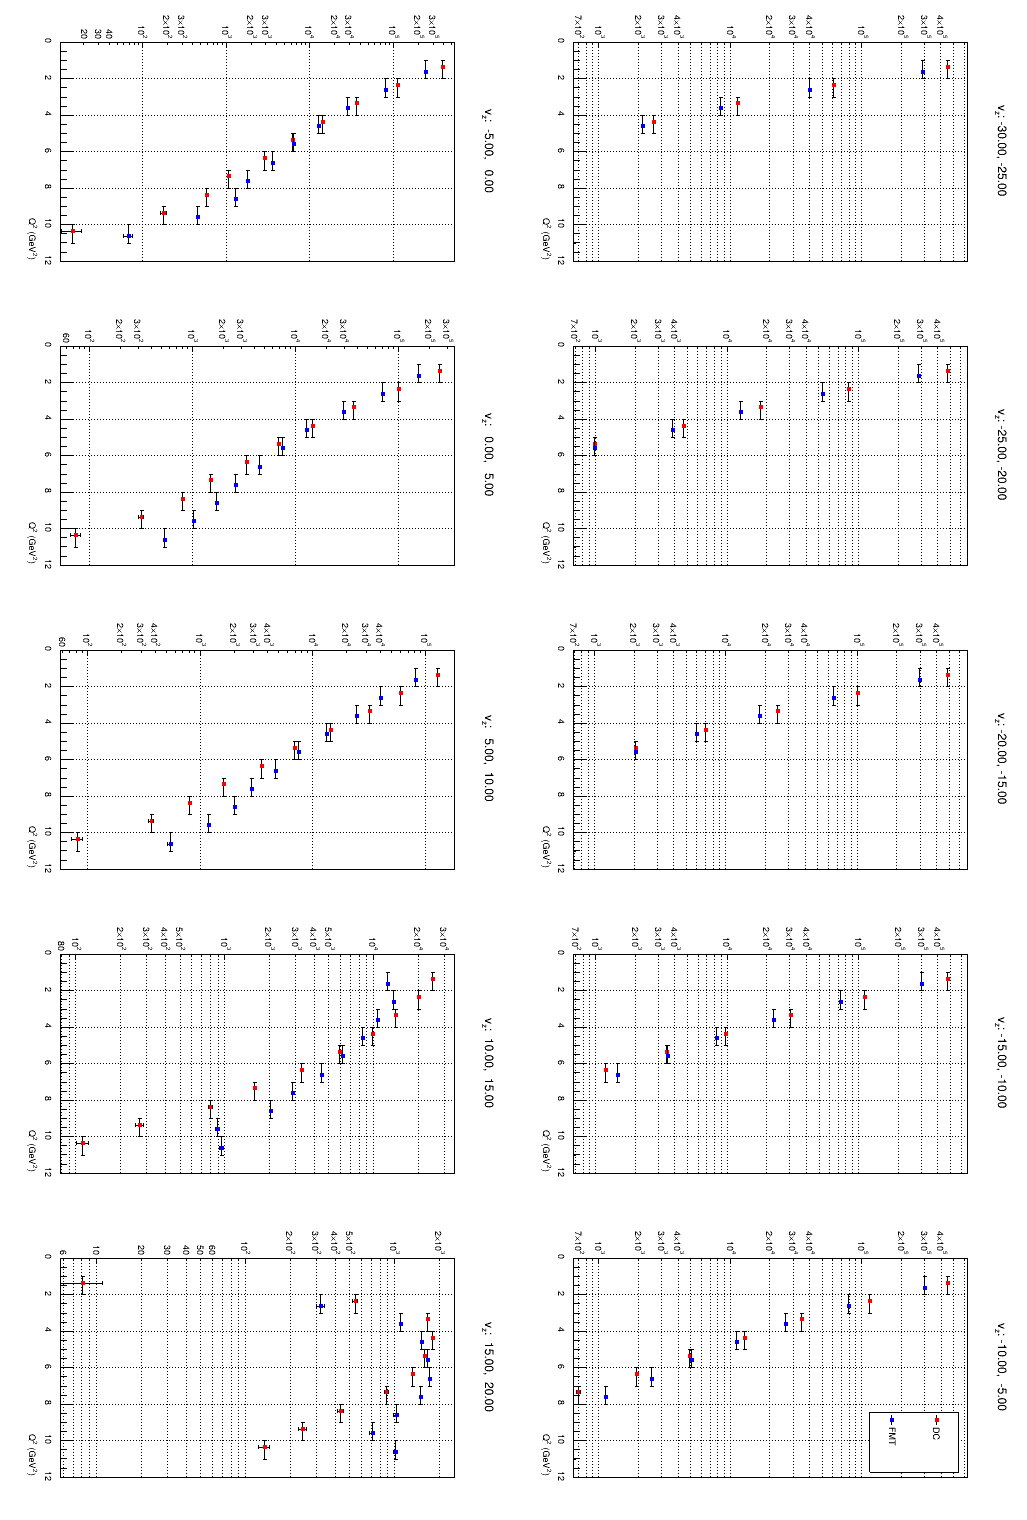
\includegraphics[width=\textwidth]{30q2_vz.png}
        \caption[Acceptance-corrected $Q^2$ separated in $v_z$ bins, run 12016]
        {Acceptance-corrected $Q^2$ detected by DC and FMT, separated in $v_z$ bins.
        Run 12016.
        The bin markers are slightly shifted in $x$ to improve legibility.}
        \floatfoot{Source: Own elaboration, using the \href{https://github.com/bleaktwig/clas12-rge-analysis}{clas12-rge-analysis} software.}
        \label{fig::14.30::q2_vz}
    \end{figure}

    % nu.
    \begin{figure}
        \centering
        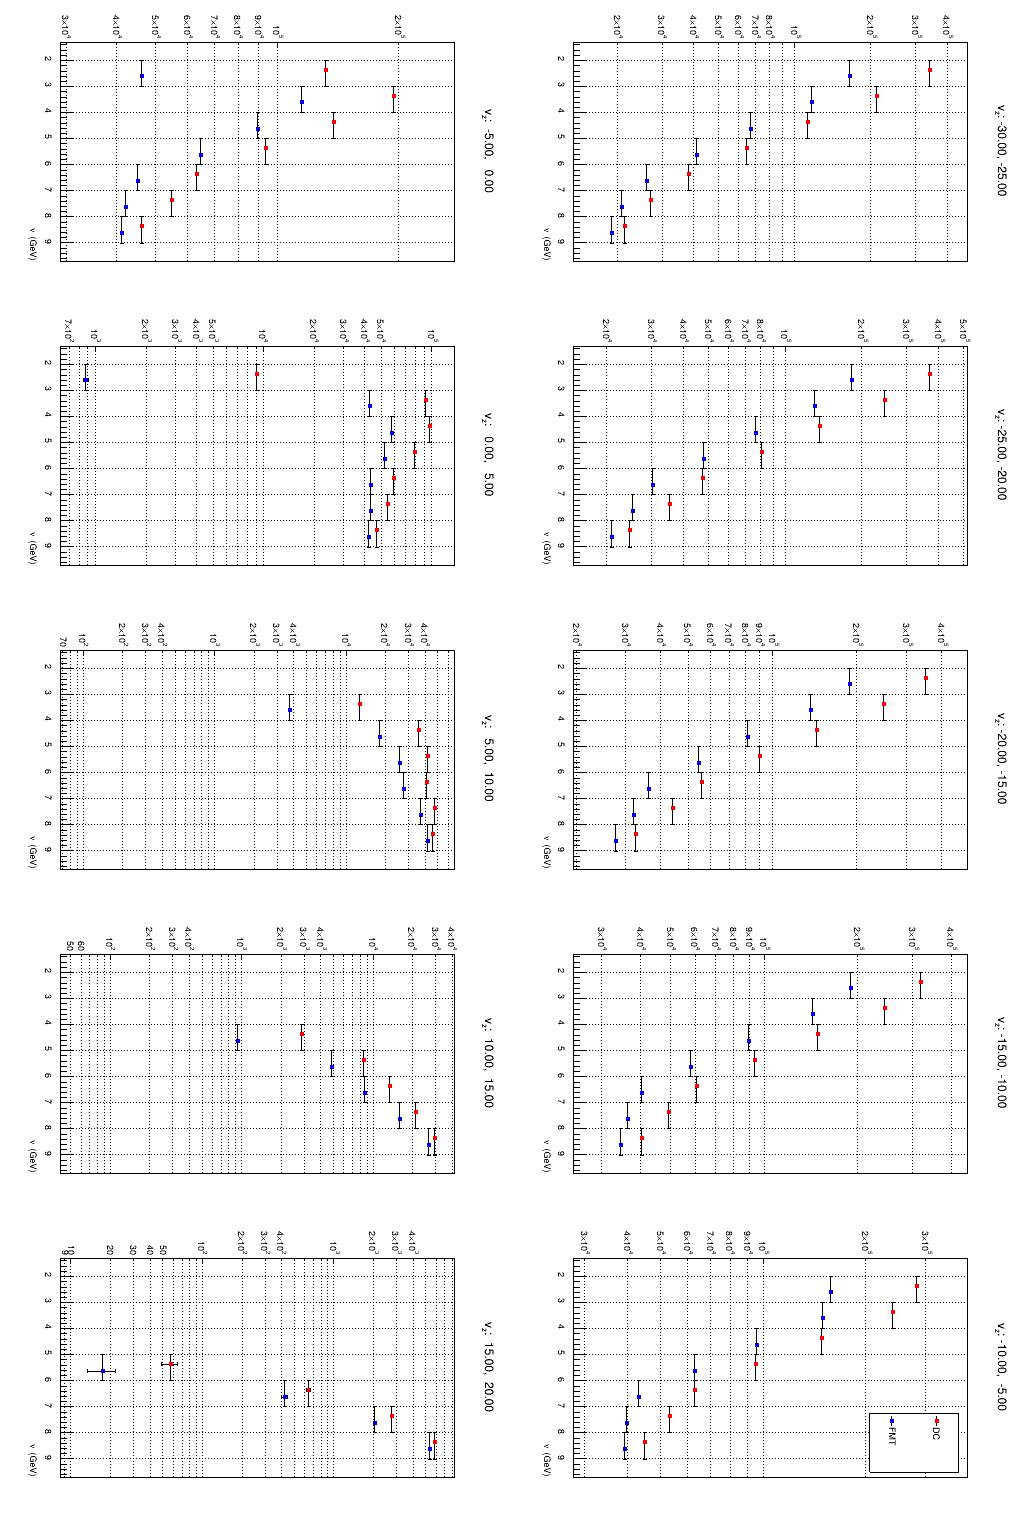
\includegraphics[width=\textwidth]{30nu_vz.png}
        \caption[Acceptance-corrected $\nu$ separated in $v_z$ bins, run 12016]
        {Acceptance-corrected $\nu$ detected by DC and FMT, separated in $v_z$ bins.
        Run 12016.
        The bin markers are slightly shifted in $x$ to improve legibility.}
        \floatfoot{Source: Own elaboration, using the \href{https://github.com/bleaktwig/clas12-rge-analysis}{clas12-rge-analysis} software.}
        \label{fig::14.30::nu_vz}
    \end{figure}

    % zh.
    \begin{figure}
        \centering
        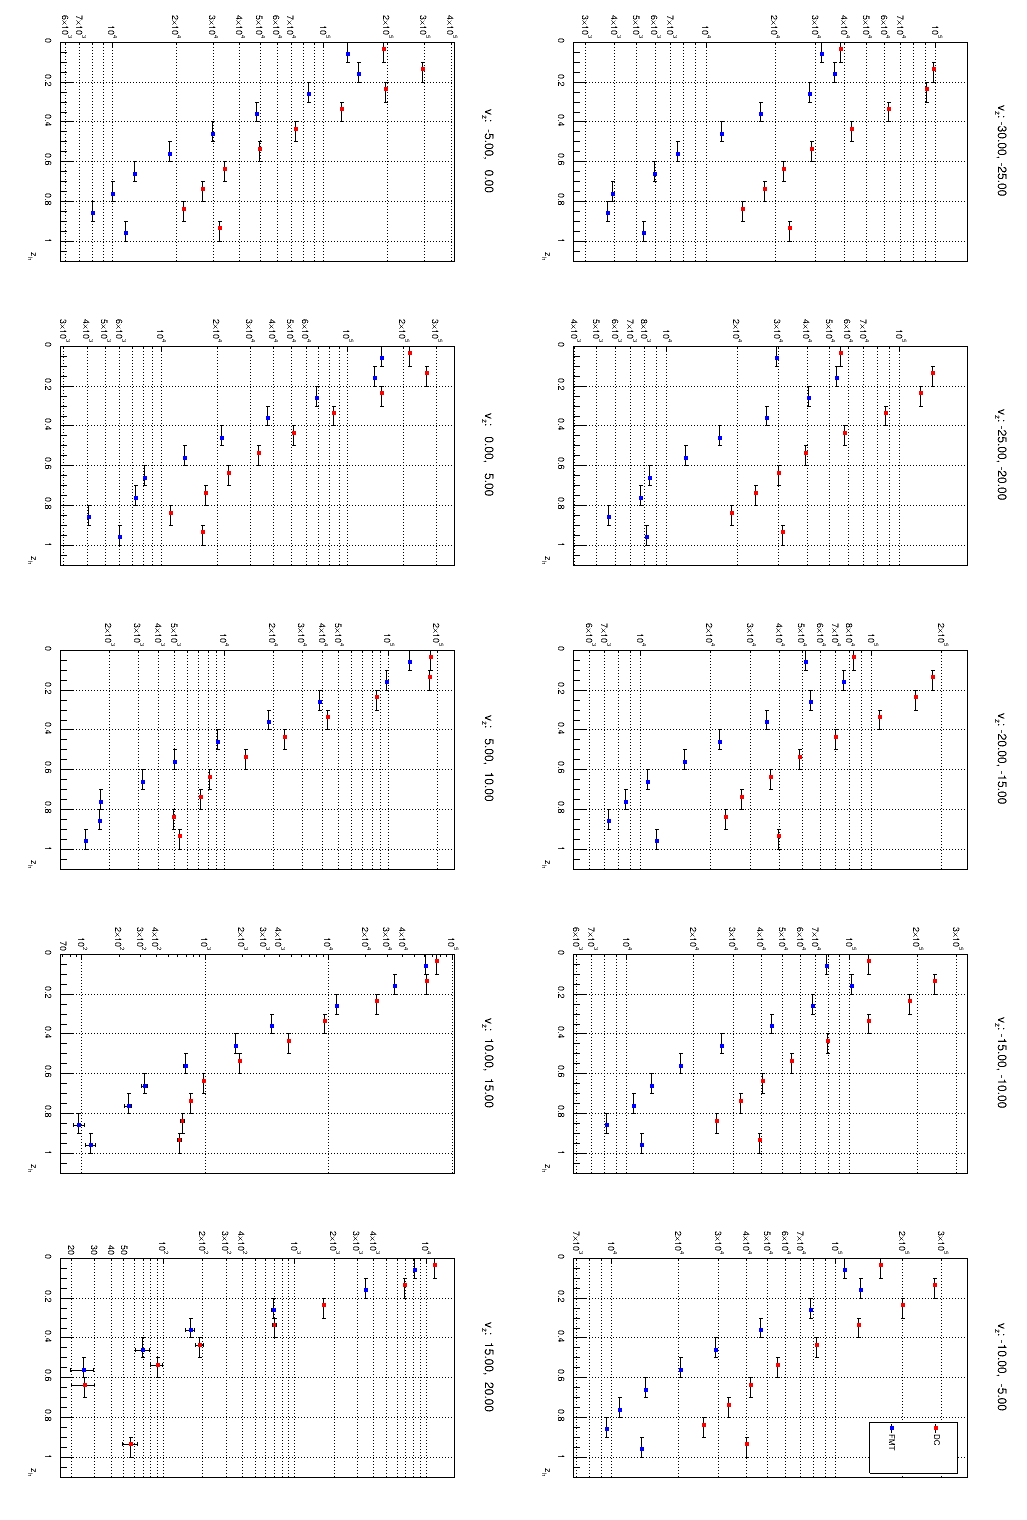
\includegraphics[width=\textwidth]{30zh_vz_211.png}
        \caption[Acceptance-corrected $z_h$ for $e^-\pi^+$ separated in $v_z$ bins, run 12016]
        {Acceptance-corrected $z_h$ for $e^-\pi^+$ detected by DC and FMT, separated in $v_z$ bins.
        Run 12016.
        The bin markers are slightly shifted in $x$ to improve legibility.}
        \floatfoot{Source: Own elaboration, using the \href{https://github.com/bleaktwig/clas12-rge-analysis}{clas12-rge-analysis} software.}
        \label{fig::14.30::zh_211_vz}
    \end{figure}

    \begin{figure}
        \centering
        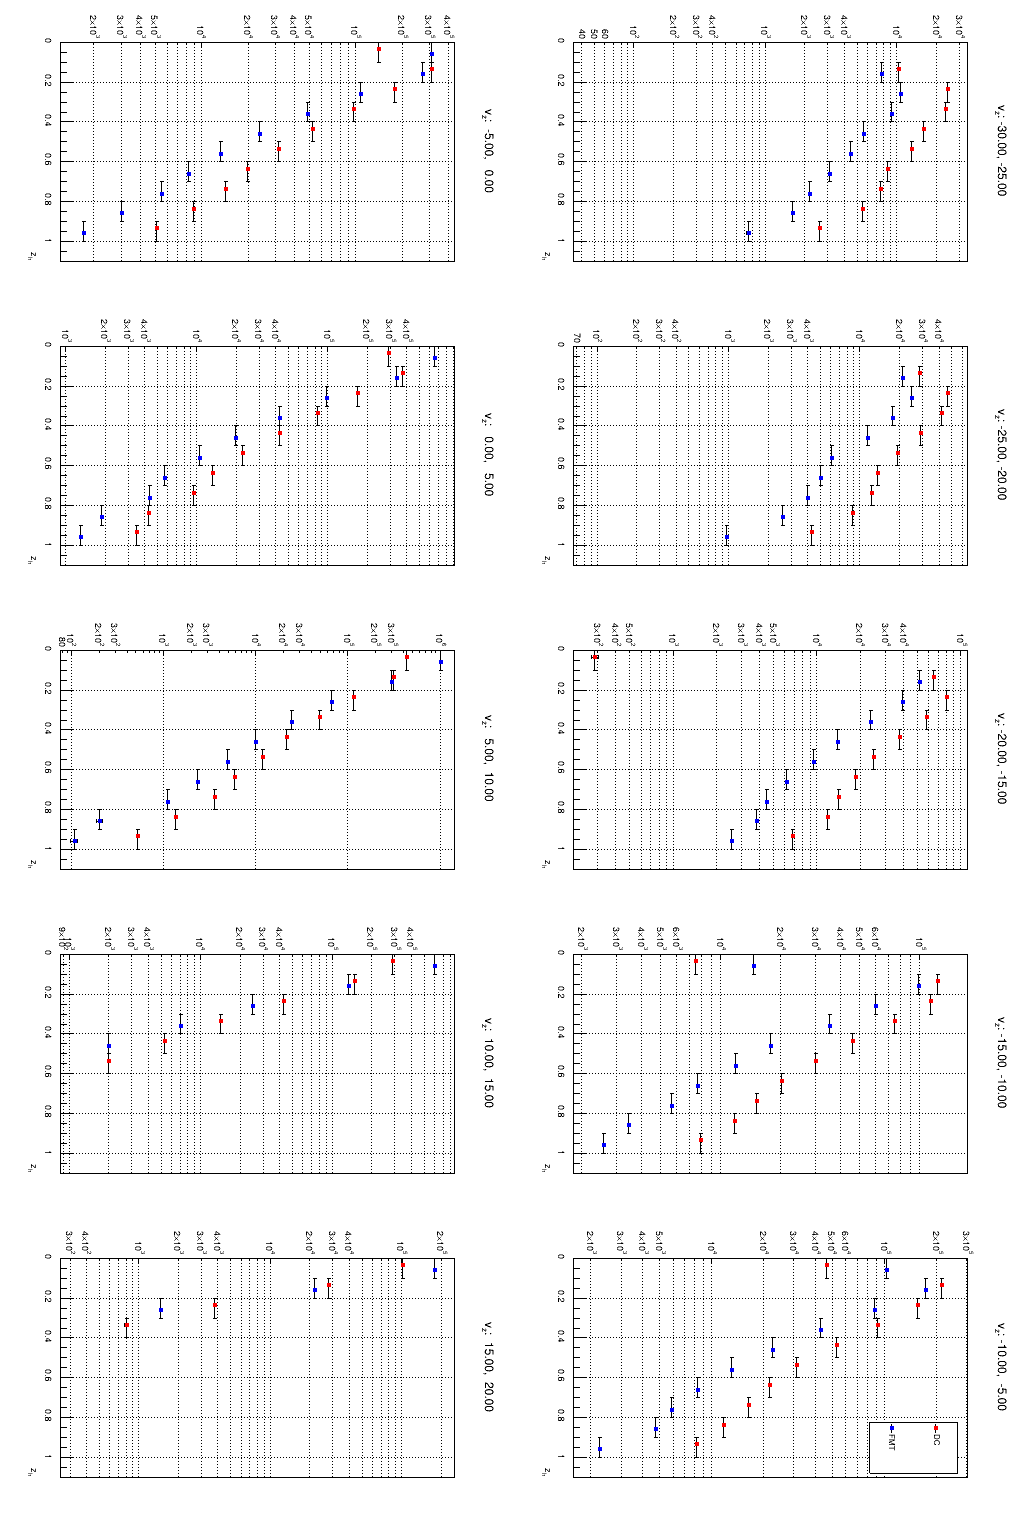
\includegraphics[width=\textwidth]{30zh_vz_-211.png}
        \caption[Acceptance-corrected $z_h$ for $e^-\pi^-$ separated in $v_z$ bins, run 12016]
        {Acceptance-corrected $z_h$ for $e^-\pi^-$ detected by DC and FMT, separated in $v_z$ bins.
        Run 12016.
        The bin markers are slightly shifted in $x$ to improve legibility.}
        \floatfoot{Source: Own elaboration, using the \href{https://github.com/bleaktwig/clas12-rge-analysis}{clas12-rge-analysis} software.}
        \label{fig::14.30::zh_-211_vz}
    \end{figure}

    % pt2.
    \begin{figure}
        \centering
        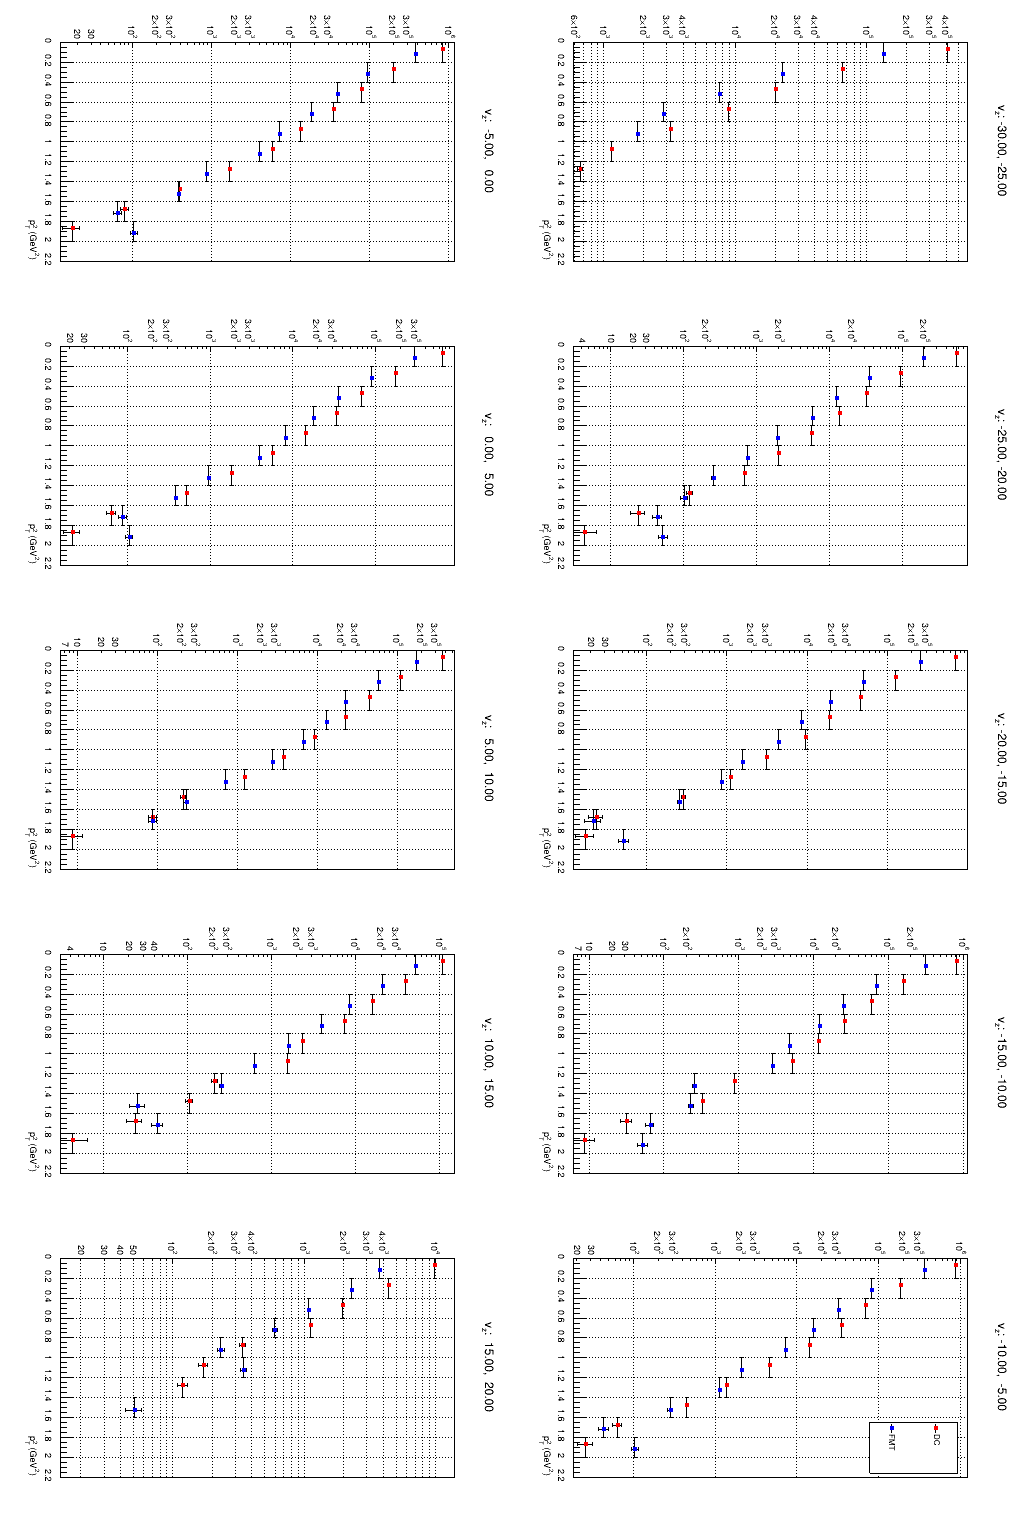
\includegraphics[width=\textwidth]{30pt2_vz_211.png}
        \caption[Acceptance-corrected $p_T^2$ for $e^-\pi^+$ separated in $v_z$ bins, run 12016]
        {Acceptance-corrected $p_T^2$ for $e^-\pi^+$ detected by DC and FMT, separated in $v_z$ bins.
        Run 12016.
        The bin markers are slightly shifted in $x$ to improve legibility.}
        \floatfoot{Source: Own elaboration, using the \href{https://github.com/bleaktwig/clas12-rge-analysis}{clas12-rge-analysis} software.}
        \label{fig::14.30::pt2_211_vz}
    \end{figure}

    \begin{figure}
        \centering
        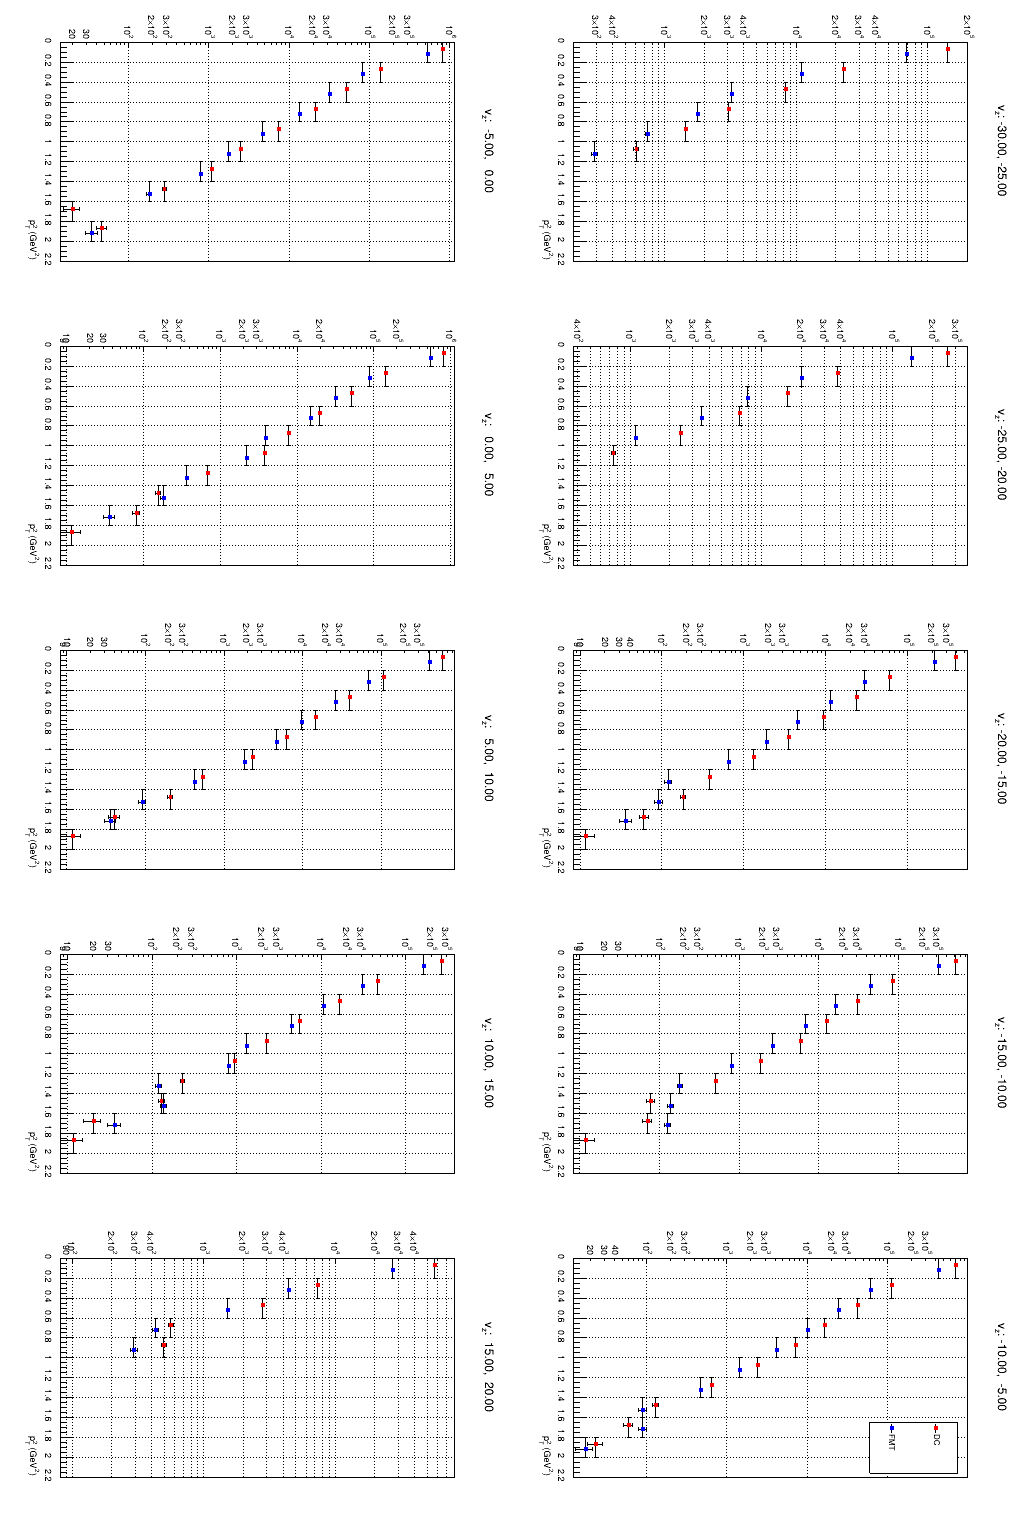
\includegraphics[width=\textwidth]{30pt2_vz_-211.png}
        \caption[Acceptance-corrected $p_T^2$ for $e^-\pi^-$ separated in $v_z$ bins, run 12016]
        {Acceptance-corrected $p_T^2$ for $e^-\pi^-$ detected by DC and FMT, separated in $v_z$ bins.
        Run 12016.
        The bin markers are slightly shifted in $x$ to improve legibility.}
        \floatfoot{Source: Own elaboration, using the \href{https://github.com/bleaktwig/clas12-rge-analysis}{clas12-rge-analysis} software.}
        \label{fig::14.30::pt2_-211_vz}
    \end{figure}

    % phipq.
    \begin{figure}
        \centering
        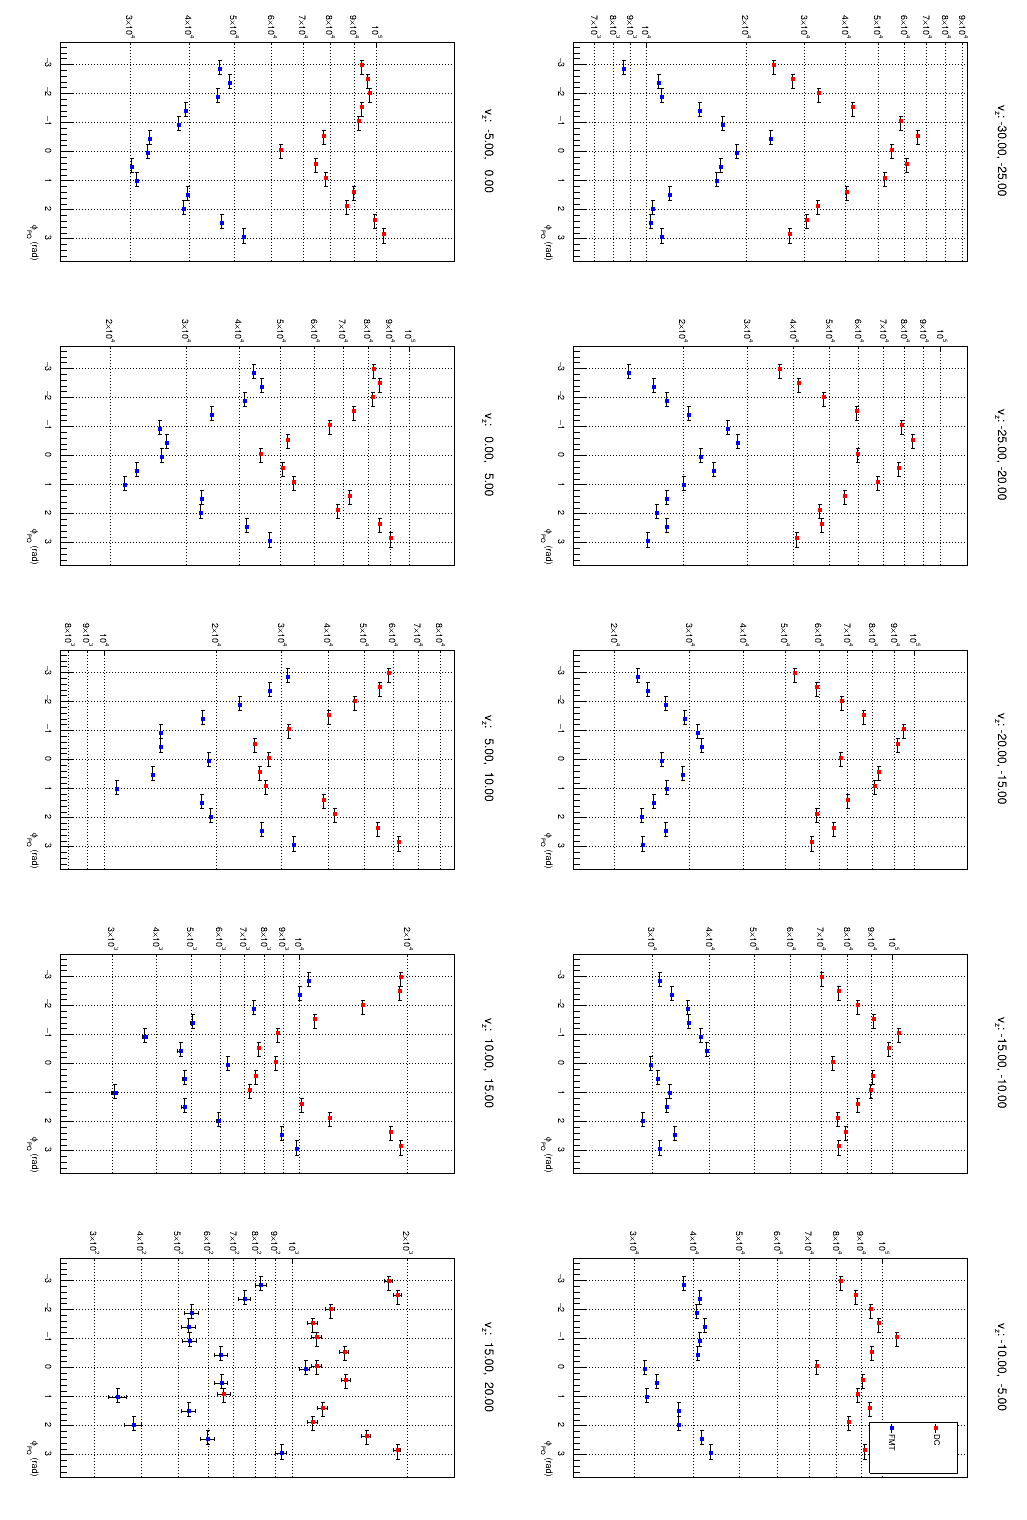
\includegraphics[width=\textwidth]{30phipq_vz_211.png}
        \caption[Acceptance-corrected $\phi_{PQ}$ for $e^-\pi^+$ separated in $v_z$ bins, run 12016]
        {Acceptance-corrected $\phi_{PQ}$ for $e^-\pi^+$ detected by DC and FMT, separated in $v_z$ bins.
        Run 12016.
        The bin markers are slightly shifted in $x$ to improve legibility.}
        \floatfoot{Source: Own elaboration, using the \href{https://github.com/bleaktwig/clas12-rge-analysis}{clas12-rge-analysis} software.}
        \label{fig::14.30::phipq_211_vz}
    \end{figure}

    \begin{figure}
        \centering
        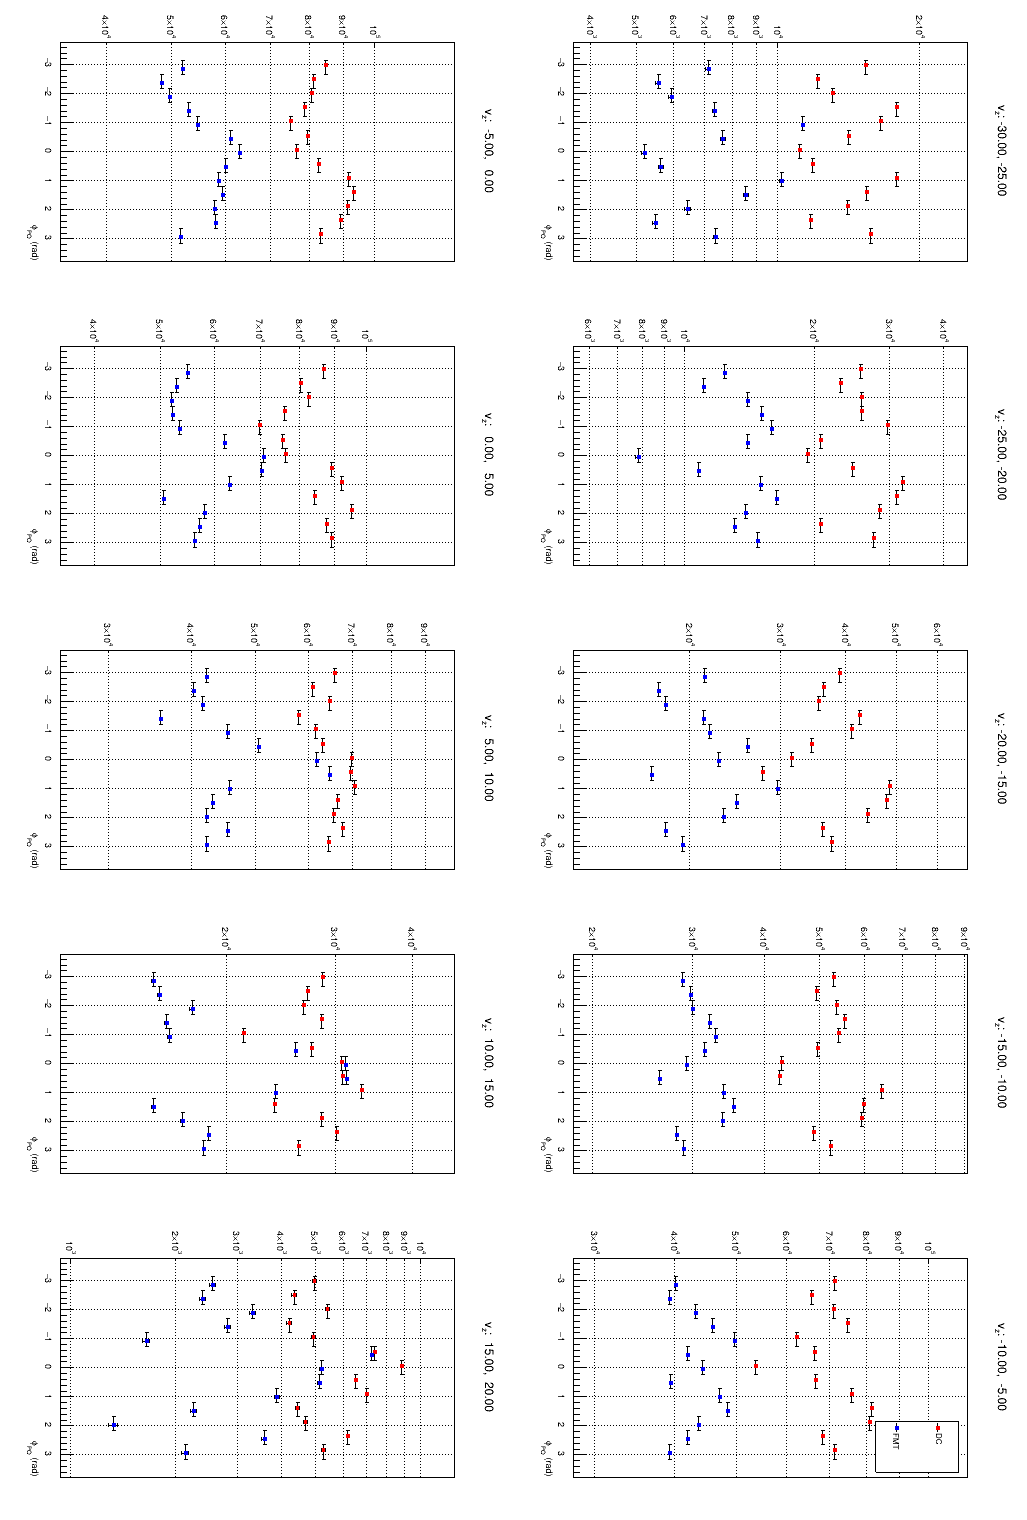
\includegraphics[width=\textwidth]{30phipq_vz_-211.png}
        \caption[Acceptance-corrected $\phi_{PQ}$ for $e^-\pi^-$ separated in $v_z$ bins, run 12016]
        {Acceptance-corrected $\phi_{PQ}$ for $e^-\pi^-$ detected by DC and FMT, separated in $v_z$ bins.
        Run 12016.
        The bin markers are slightly shifted in $x$ to improve legibility.}
        \floatfoot{Source: Own elaboration, using the \href{https://github.com/bleaktwig/clas12-rge-analysis}{clas12-rge-analysis} software.}
        \label{fig::14.30::phipq_-211_vz}
    \end{figure}
